\chapter{Kajian Literasi}
\section{Pengenalan}


Di Malaysia, Pendidikan 4.0 telah mula diterapkan dalam sistem pendidikan sejak 2018 dengan tema \textit{Higher Education 4.0: Knowledge, Industry, and Humanity}. Pelbagai dasar dan strategi telah diimplementasikan, termasuk Pelan Pembangunan Pendidikan Malaysia (MEB) 2013--2025 yang menekankan pendidikan berkualiti serta pembangunan pelajar yang mampu bersaing dalam industri masa depan. Kementerian Pendidikan Malaysia (MOE) juga telah memperkenalkan teknologi seperti \textit{AR}, \textit{VR}, \textit{artificial intelligence (AI)}, dan \textit{Internet of Things (IoT)} dalam pengajaran bagi memastikan pelajar memperoleh kemahiran digital yang diperlukan.(Idris Skloul Ibrahim,2022)\\

\hspace{1cm}Dalam konteks ini, \textit{Bahasa Inggeris} memainkan peranan yang sangat penting dalam \textit{Pendidikan 4.0}. Pelaksanaan \textit{Common European Framework of Reference for Languages (CEFR)} di Malaysia bertujuan untuk meningkatkan komunikasi pelajar dalam \textit{Bahasa Inggeris} melalui pendekatan yang lebih interaktif dan berbentuk praktikal. Walau bagaimanapun, kajian menunjukkan bahawa ramai pelajar Malaysia menghadapi kesukaran dalam pembelajaran bahasa ini akibat kurangnya penggunaan teknologi dalam pengajaran \cite{zainuddin2021}. Teknologi AR berpotensi meningkatkan pengalaman pembelajaran dengan menyediakan simulasi interaktif yang membantu pelajar memahami konsep bahasa dengan lebih baik.(Aditi Chaudhary ,. et al 2022)\\

\hspace{1cm}Kajian ini bertujuan untuk meneroka penggunaan AR sebagai alat dalam pendidikan bahasa serta mengenal pasti batasan teknologi ini dalam pembelajaran Bahasa Inggeris sebagai Bahasa Kedua (ESL)(Izia ,.et al 2024)  Dengan memahami kelebihan dan kekangan AR dalam bilik darjah, penyelidikan ini dapat memberikan panduan kepada pendidik dan pembuat dasar dalam mengintegrasikan teknologi ini dalam kurikulum pendidikan.Bab ini membincangkan konsep literasi dalam konteks pendidikan prasekolah serta potensi penggunaan \textit{Augmented Reality }(AR) sebagai alat inovatif untuk memperkayakan pengalaman pembelajaran huruf dalam kalangan murid prasekolah.Kajian lampau telah menunjukkan bahawa meskipun kaedah pembelajaran tradisional seperti buku teks dan latihan bertulis masih meluas digunakan, ia menghadapi pelbagai cabaran dalam memastikan murid benar-benar menguasai, mengingati dan berinteraksi dengan konsep literasi secara menyeluruh ( Amy Debbané  et al., 2023). Seiring perkembangan teknologi dan permintaan pendidikan abad ke-21, integrasi teknologi seperti AR dalam literasi awal semakin menjadi tumpuan dalam bidang akademik dan amalan pendidikan, memandangkan potensinya untuk menyediakan pendekatan yang lebih interaktif, menyeronokkan, serta efektif dalam pembelajaran huruf dan kemahiran membaca (Azuma, 1997; Chen et al., 2020).

\section{Teori New Literacy Studies (NLS)}

\subsection{Pengenalan kepada NLS}
Dalam era pendidikan moden, literasi tidak lagi terhad kepada kemahiran membaca dan menulis secara mekanikal semata-mata, tetapi telah berkembang menjadi satu amalan sosial dan budaya yang dipengaruhi oleh kemajuan teknologi, interaksi antara individu, serta perkembangan dunia digital (Gee, 1999; Kementerian Pendidikan Malaysia, 2013). Perubahan ini menuntut murid untuk bukan sahaja menguasai literasi asas, tetapi juga kebolehan menggunakan teknologi dan berinteraksi dalam pelbagai konteks pembelajaran abad ke-21 (UNESCO, 2022).

\hspace{1cm}James Paul Gee (1999) merupakan salah seorang sarjana yang memperkenalkan \textit{New Literacy Studies} (NLS), yang menekankan bahawa literasi bukan hanya merujuk kepada keupayaan membaca dan menulis secara formal, tetapi juga bagaimana seseorang menggunakan bahasa dan komunikasi dalam situasi sosial yang lebih luas.

\hspace{1cm}Street (2003) pula memperkukuhkan konsep ini dengan menyatakan bahawa literasi bukan sekadar kecekapan kognitif, tetapi turut berkait rapat dengan budaya, masyarakat, dan teknologi. Kajian NLS menunjukkan bahawa literasi berkembang mengikut keperluan sosial, di mana seseorang bukan hanya memahami perkataan, tetapi juga menggunakannya, menyesuaikan diri, serta berinteraksi dengan maklumat dalam konteks dunia sebenar.

\subsection{{Implikasi NLS dalam Pendidikan Moden}}
Teknologi \textit{Augmented Reality} (AR) memainkan peranan penting dalam mengukuhkan pendekatan\textit{ New Literacy Studies}, kerana ia mengubah cara pelajar berinteraksi dengan bahan pembelajaran.

Pembelajaran huruf tidak lagi terbatas kepada format dua dimensi (2D) yang statik, tetapi telah berkembang kepada bentuk tiga dimensi (3D) yang lebih interaktif. Dengan teknologi AR, pelajar dapat melihat, menyentuh, dan mendengar huruf serta perkataan dalam cara yang lebih dinamik, seterusnya membantu mereka memahami konsep dengan lebih mendalam.

Tambahan pula, AR membolehkan murid memahami bukan sahaja bentuk huruf, tetapi juga cara huruf digunakan dalam kehidupan sebenar melalui visualisasi dan animasi. Pendekatan ini selari dengan konsep NLS, yang menekankan bahawa literasi moden bukan sekadar kemahiran teknikal, tetapi turut diperkaya dengan konteks sosial dan teknologi.



\subsection{Kajian Terdahulu Mengenai NLS dan AR dalam Pendidikan}
Beberapa kajian terdahulu telah membuktikan hubungan antara \textit{New Literacy Studies }dan penggunaan AR dalam pendidikan, seperti yang ditunjukkan dalam Jadual2.1


\begin{table}[htbp]
    \centering
    \caption{Hubungan antara New Literacy Studies dan penggunaan AR dalam pendidikan}
    \label{tab:literacy-ar}
    \begin{tabularx}{\textwidth}{l l X}
        \toprule
        \textbf{Kajian} & \textbf{Fokus Kajian} & \textbf{Hasil Kajian} \\
        \midrule
        Vrunda (2023) & Literasi sebagai praktik sosial & Literasi bukan hanya kemahiran membaca tetapi interaksi dengan budaya dan masyarakat. \\
        Cheng Zhao (2024) & Literasi dan digitalisasi & Literasi berkembang dengan kemajuan teknologi dan persekitaran sosial. \\
       Md Naimul Hoque (2024) & Kesan AR terhadap literasi & AR meningkatkan pemahaman konsep dengan interaksi visual dan auditori. \\
        Rahmawati et al. (2022) & AR dalam literasi awal & Murid prasekolah lebih cepat mengenali huruf dengan bantuan AR interaktif. \\
        \bottomrule
    \end{tabularx}
\end{table}



\subsection{Implikasi kepada Kajian Ini}
Kajian ini menerapkan prinsip New Literacy Studies (NLS) melalui pembangunan aplikasi \textit{AR Alphabets}, bagi menilai bagaimana teknologi ini dapat membantu meningkatkan literasi awal murid prasekolah secara interaktif dan visual.Teknologi \textit{Augmented Reality} (AR) berfungsi sebagai pelengkap kepada pendekatan NLS, membolehkan murid berinteraksi dengan huruf dan bunyi dalam bentuk yang lebih menarik dan berkesan. Kajian ini akan membandingkan keberkesanan AR dengan kaedah pembelajaran tradisional, sejajar dengan pandangan NLS yang menekankan bahawa literasi moden perlu berkembang selaras dengan perubahan teknologi.

\subsection{Kesimpulan}
Bab ini telah mengembangkan Teori \textit{New Literacy Studies} (NLS) secara lebih mendalam dan kritikal, menjelaskan bahawa literasi bukan sekadar kemahiran membaca dan menulis, tetapi juga praktik sosial yang diperkaya dengan teknologi seperti AR.Kajian ini akan meneliti bagaimana integrasi AR dapat memperkukuhkan pembelajaran literasi awal, memberikan pengalaman pembelajaran yang lebih dinamik, interaktif, dan efektif bagi murid prasekolah.

\section{Multiliteracies dan Literasi Digital}

Dalam dunia pendidikan moden, konsep literasi tidak lagi terbatas kepada bacaan dan penulisan dalam bentuk teks sahaja, tetapi telah berkembang kepada pelbagai bentuk komunikasi yang lebih luas dan kompleks.

Kalantzis dan Cope (2000) memperkenalkan konsep \textit{Multiliteracies}, yang memberi tumpuan kepada cara manusia berkomunikasi melalui pelbagai saluran, termasuk visual, auditori, digital, dan multimodal. Konsep ini berkembang selaras dengan perubahan dalam cara maklumat disampaikan dan diterima oleh masyarakat moden.

\hspace{1cm}Dengan kepesatan teknologi dan globalisasi, pembelajaran tidak lagi tertumpu kepada buku teks dan tulisan sahaja, tetapi merangkumi pelbagai medium komunikasi digital, seperti grafik, video, animasi, dan interaksi teknologi.
Pendekatan\textit{ Multiliteracies }menekankan bahawa pelajar tidak hanya berinteraksi dengan teks bertulis, tetapi juga dengan imej, bunyi, animasi, serta teknologi digital, yang menjadi sebahagian daripada pengalaman pembelajaran mereka. Dalam dunia yang dipenuhi dengan maklumat digital, pelajar perlu menguasai bukan sahaja literasi tradisional, tetapi juga kemahiran teknologi untuk memahami dan memproses maklumat dengan lebih efektif dan efisien.

\subsection{Multiliteracies dan Literasi Digital dalam Konteks Pendidikan}
Literasi digital merujuk kepada keupayaan seseorang dalam memahami, menilai, dan menggunakan teknologi untuk mengakses dan menganalisis maklumat (UNESCO, 2022).

Dalam sistem pendidikan yang semakin bergantung kepada teknologi, pelajar perlu menguasai kemahiran digital bagi memahami dunia yang semakin pantas dan interaktif. Kajian menunjukkan bahawa pelajar yang mempunyai literasi digital yang tinggi lebih cenderung untuk memahami konsep pembelajaran dengan lebih mendalam dan mampu menyesuaikan diri dengan pelbagai bentuk komunikasi Buckingham, (2008).

Teknologi seperti Augmented Reality (AR) dan Virtual Reality (VR) kini digunakan untuk memperkukuhkan literasi digital, dengan membolehkan pelajar berinteraksi dengan konsep pembelajaran dalam persekitaran maya yang lebih realistik Keqin Li, (2)024
Sebagai sebahagian daripada perkembangan teknologi pendidikan, literasi digital bukan sahaja penting untuk mencapai kefahaman akademik, tetapi juga bagi memperluaskan keupayaan pelajar dalam berkomunikasi dan menyelesaikan masalah dalam dunia sebenar.

\subsection{Augmented Reality (AR) sebagai Alat Pembelajaran Multimodal}
Teknologi Augmented Reality (AR) memainkan peranan penting dalam perkembangan konsep Multiliteracies, kerana ia membolehkan pelajar berinteraksi dengan bahan pembelajaran melalui pelbagai saluran komunikasi digital.(Zhang et al., 2025)

AR dikategorikan sebagai alat pembelajaran multimodal, kerana ia melibatkan visualisasi 3D, animasi, bunyi, dan interaktiviti, sejajar dengan pendekatan multiliterasi dalam pendidikan moden.(Ashvini Varatharaj  et al (2024)

AR membolehkan pelajar melihat objek maya dalam persekitaran fizikal, yang memberikan mereka pengalaman pembelajaran yang lebih immersif dan realistik. Dalam konteks literasi awal, AR membantu murid mengenali huruf bukan hanya sebagai simbol statik, tetapi sebagai elemen yang hidup, boleh disentuh, serta didengar.

Kajian menunjukkan bahawa pelajar yang menggunakan AR dalam pembelajaran cenderung untuk lebih cepat memahami konsep, berbanding mereka yang menggunakan kaedah tradisional Billinghurst \& Dünser, (2012).

\subsection{Kajian Terdahulu Mengenai Multiliteracies dan Literasi Digital}
Berikut adalah beberapa kajian terdahulu yang menyokong perkembangan konsep Multiliteracies dan Literasi Digital dalam pendidikan, seperti yang ditunjukkan dalam Jadual~\ref{tab:multiliteracies}
\section{Hubungan antara Multiliteracies dan Literasi Digital dalam Pendidikan}

\begin{table}[htbp]
    \centering
    \caption{Hubungan antara Multiliteracies dan Literasi Digital dalam Pendidikan}
    \label{tab:multiliteracies}
    \begin{tabular}{@{}p{3cm} p{4cm} p{6cm}@{}}
        \toprule
        \textbf{Kajian} & \textbf{Fokus Kajian} & \textbf{Hasil Kajian} \\
        \midrule
        Md Naimul Hoque (2023) & Konsep Multiliteracies & Literasi moden merangkumi visual, auditori, dan komunikasi digital. \\
       Adrien de Jarmy(2024) & Literasi Digital & Pelajar dengan kemahiran literasi digital memahami maklumat dengan lebih baik. \\
        Xinji Mai et al (2024) & AR dalam pembelajaran & AR meningkatkan pemahaman konsep melalui pembelajaran multimodal. \\
       Himmet Toprak Kesgin, et al. (2024) & Interaksi AR dalam pendidikan & Pelajar lebih berkesan memahami konsep pembelajaran apabila menggunakan AR. \\
        \bottomrule
    \end{tabular}
\end{table}

\section{Literasi Digital dan Teknologi Pendidikan}

\subsection{Pengenalan kepada Literasi Digital}

Dalam era teknologi moden, literasi tidak lagi terbatas kepada keupayaan membaca dan menulis secara konvensional, tetapi telah berkembang kepada keupayaan mengakses, menilai, dan memahami maklumat digital secara kritikal. Literasi digital menjadi semakin penting kerana dunia pendidikan dan industri kini bergantung kepada teknologi sebagai medium komunikasi dan pembelajaran utama (UNESCO, 2022).

\hspace{1cm}Sourojit Ghosh(2024), literasi digital merangkumi kemahiran mencari, menilai, dan menggunakan maklumat yang diperoleh melalui teknologi. Ini bermakna pelajar bukan sahaja perlu tahu membaca teks tetapi juga memahami kandungan multimedia, menilai kesahihan maklumat, dan menggunakannya secara efektif dalam kehidupan seharian.

\subsection{Kepentingan Literasi Digital dalam Kurikulum Pendidikan}

UNESCO (2022) menegaskan bahawa literasi digital perlu menjadi asas utama dalam kurikulum pendidikan kerana ia membantu pelajar berinteraksi dengan maklumat secara aktif dan bermakna. Kementerian Pendidikan Malaysia (KPM) turut menekankan kepentingan penggunaan teknologi dalam sistem pendidikan, sejajar dengan Pelan Pembangunan Pendidikan Malaysia (PPPM 2013-2025).

\hspace{1cm}Dalam pendidikan prasekolah, literasi digital membantu murid beradaptasi dengan teknologi sejak usia muda, membolehkan mereka mengembangkan daya fikir yang lebih kreatif serta memahami maklumat secara visual dan interaktif.

\hspace{1cm}Kajian menunjukkan bahawa pelajar yang mempunyai literasi digital yang tinggi lebih berupaya memahami konsep pembelajaran dengan mendalam dan mampu menyesuaikan diri dengan persekitaran teknologi yang berubah dengan pantas (Kalantzis \& Cope, 2000).


\subsection{Literasi Berkaitan Augmented Reality (AR)}
Augmented Reality (AR) merupakan teknologi yang menggabungkan elemen digital ke dalam dunia nyata, membolehkan pengguna berinteraksi dengan objek maya dalam persekitaran fizikal (Azuma, 1997). Dalam konteks pendidikan, AR digunakan untuk memperkaya pengalaman pembelajaran, menjadikan konsep abstrak lebih mudah difahami melalui visualisasi interaktif (Billinghurst \& Dünser, 2012). Kajian menunjukkan bahawa AR dapat meningkatkan pemahaman pelajar, motivasi pembelajaran, dan daya ingatan, serta membolehkan pelajar mengalami konsep pembelajaran dengan lebih realistik (Wu et al., 2013).

\subsection{Sejarah Perkembangan Augmented Reality (AR)}
Teknologi AR telah berkembang sejak beberapa dekad lalu, bermula dengan konsep asas sehingga aplikasi moden dalam pelbagai bidang. Jadual 2-4 menunjukkan perkembangan AR:

\begin{table}
\centering
\caption{Literasi Berkaitan Augmented Reality }
\label{tab:my_table}
\begin{tabular}{l >{\raggedright\arraybackslash}p{12cm}}
\hline
\textbf{\textbf{Tahun}} & \textbf{\textbf{Peristiwa Penting}} \\
\hline
\textbf{\textbf{1968}} & Ivan Sutherland mencipta \textbf{\textbf{head-mounted display pertama}}, dikenali sebagai "The Sword of Damocles". \\
\textbf{\textbf{1990}} & Tom Caudell, penyelidik Boeing, mencipta istilah \textbf{\textbf{Augmented Reality}}. \\
\textbf{\textbf{1992}} & Louis Rosenburg membangunkan sistem AR pertama yang berfungsi sepenuhnya, dikenali sebagai \textbf{\textbf{Virtual Fixtures}}. \\
\textbf{\textbf{2000}} & ARToolkit diperkenalkan sebagai alat pembangunan AR sumber terbuka. \\
\textbf{\textbf{2013}} & Google Glass dilancarkan sebagai salah satu peranti AR komersial pertama. \\
\textbf{\textbf{2020}} & Apple memperkenalkan teknologi AR yang lebih maju dalam iPhone dan iPad. \\
\hline
\end{tabular}
\end{table}
\begin{figure}[H]
    \centering
    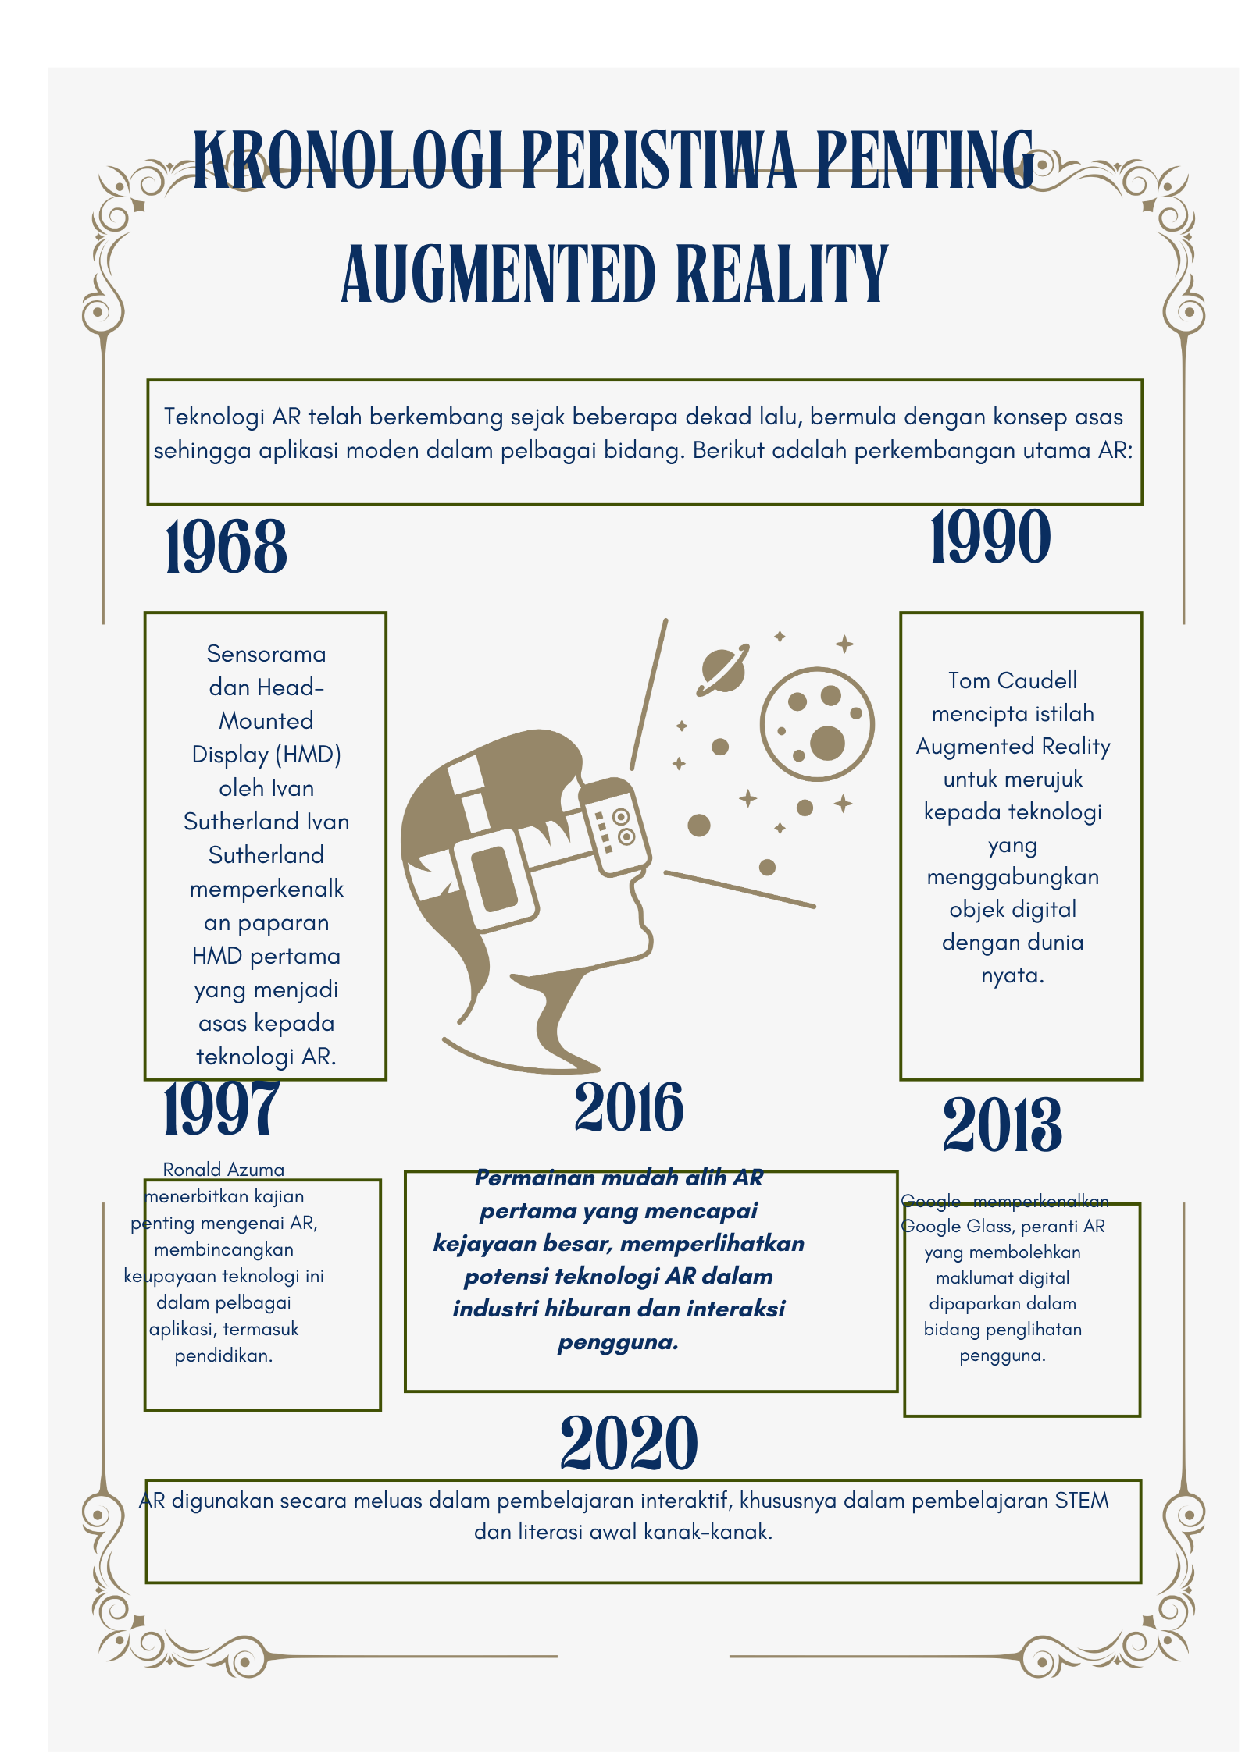
\includegraphics[width=1\linewidth]{info.pdf}
    \caption{Kronologi Peristiwa Penting Augmented Reality}
    \label{fig:enter-label}
\end{figure}
\begin{itemize}
    \item Meningkatkan pemahaman konsep abstrak melalui visualisasi 3D.
    \item Menggalakkan pembelajaran kendiri dengan akses kepada kandungan digital yang lebih menarik.
    \item Memudahkan guru menyampaikan konsep yang lebih sukar dengan lebih jelas.
    \item Meningkatkan motivasi dan daya ingatan pelajar melalui interaksi langsung dengan bahan pembelajaran.
\end{itemize}

Kajian menunjukkan bahawa AR boleh digunakan dalam pelbagai bidang pendidikan, termasuk sains, matematik, bahasa, dan sejarah.

\subsection{{Kajian Terdahulu mengenai AR dalam Pendidikan}}

Jadual 2.5 menunjukkan kajian terdahulu yang membincangkan kesan penggunaan AR dalam pendidikan:

\begin{table}[ht]
    \centering
    \caption{Jadual 2-5: Kajian Terdahulu Mengenai AR dalam Pendidikan}
    \begin{tabular}{@{}>{\raggedright\arraybackslash}p{7cm}>{\raggedright\arraybackslash}p{7cm}@{}}
        \toprule
        \textbf{Kajian} & \textbf{Hasil Kajian} \\
        \midrule
        Sehkar Fayda-Kinik (2023) & AR meningkatkan pemahaman dan motivasi pelajar. \\
        Yiannis Koumpouros (2024) & AR membantu pelajar memahami konsep dengan lebih mendalam. \\
        Lampropoulos et al. (2022) & AR meningkatkan penglibatan dan prestasi akademik pelajar. \\
        \bottomrule
    \end{tabular}
\end{table}

\subsection{Kajian lepas berkaitan penggunaan teknologi Augmented Reality (AR)}

Jadual~\ref{2.9} menunjukkan ringkasan sepuluh kajian lepas berkaitan penggunaan teknologi Augmented Reality (AR) dalam pendidikan sepanjang lima tahun terkini, khususnya dari segi impak terhadap motivasi, penumpuan, dan pencapaian pelajar.


\begin{table}[ht]
    \centering
    \caption{Ringkasan Dapatan Kajian Terkini}
    \begin{tabular}{cl>{\raggedright\arraybackslash}p{0.16\linewidth}>{\raggedright\arraybackslash}p{0.54\linewidth}}
        \toprule
        Bil & Tahun & Penulis & Dapatan \\
        \midrule
        1 & 2023 & Gunalan et al. & Meningkatkan motivasi dan tumpuan murid melalui visual interaktif dan aktiviti permainan. \\
        2 & 2022 & Lin et al. & Meningkatkan penumpuan dan pencapaian murid berbanding kaedah tradisional. \\
        3 & 2021 & Gunawan et al. & Meningkatkan motivasi intrinsik dan pencapaian ujian pelajar. \\
        4 & 2020 & Sánchez et al. & Meningkatkan tumpuan dan ingatan pelajar. \\
        5 & 2019 & Norazlina et al. & Peningkatan motivasi dan pencapaian murid dalam pengenalan huruf. \\
        6 & 2023 & Cao \& Yu & Sikap dan pencapaian lebih tinggi, tiada perbezaan signifikan motivasi. \\
        7 & 2025 & Ruijia et al. & Meningkatkan motivasi melalui pengalaman pembelajaran imersif. \\
        8 & 2023 & Özeren \& Top & Meningkatkan pencapaian akademik dan motivasi berbanding tradisional. \\
        9 & 2022 & Goharinejad et al. & Mengurangkan defisit perhatian dan meningkatkan pembelajaran. \\
        10 & 2023 & Vidak et al. & Membantu visualisasi konsep abstrak dan meningkatkan pencapaian pelajar. \\
        \bottomrule
    \end{tabular}
\end{table}

\section{\textbf{PERKEMBANGAN LITERASI AWAL KANAK-KANAK}}

Literasi awal merujuk kepada kebolehan asas kanak-kanak untuk mengenal huruf, memahami fonetik dan membina hubungan antara simbol dan bunyi.

\subsection{ Teknologi Dalam Pendidikan Prasekolah}

Dalam era Revolusi Industri 4.0, pendidikan prasekolah tidak terkecuali daripada menerima impak transformasi digital. Teknologi pendidikan telah diperkenalkan secara meluas di peringkat prasekolah.

\begin{table}[htbp]
    \centering
    \caption{Kajian Literatur mengenai Integrasi Augmented Reality (AR) dalam Pendidikan Bahasa}
    \begin{tabular}{p{4cm} p{10cm}}
        \toprule
        \textbf{Pengarang} & \textbf{Hasil Kajian} \\
        \midrule
        Ibrahim et al. (2018) & Teknologi AR menyediakan pengalaman pembelajaran imersif dan persekitaran pembelajaran yang menyeronokkan. \\
        Taskiran (2019) & Hasil soal selidik menunjukkan pembelajaran berasaskan AR lebih menyeronokkan dan memberi motivasi. \\
        Xu et al. (2019) & AR meningkatkan perhatian serta keterujaan pelajar dalam kelas ESL. \\
        Ji \& Shin (2019) & AR meningkatkan minat dan rasa ingin tahu pelajar, sekaligus memperkukuhkan motivasi dalam pembelajaran bahasa. \\
        Yaacob et al. (2019) & AR berkesan dalam meningkatkan pembelajaran kosa kata serta mengekalkan tahap motivasi yang tinggi. \\
        Chang et al. (2020) & Hasil kajian menunjukkan AR meningkatkan kepekatan, keyakinan, dan menyediakan senario pembelajaran yang hampir kepada realiti. \\
        Tsai (2020) & Pembelajaran kosa kata berasaskan AR lebih berkesan berbanding kaedah tradisional. \\
        Afnan et al. (2021) & Motivasi dan prestasi pelajar meningkat dengan penggunaan teknik pembelajaran berasaskan AR. \\
        Jalaluddin et al. (2021) & MAVR ialah alat interaktif yang berkesan dalam pembelajaran kosa kata Inggeris sebagai Bahasa Kedua (ESL). \\
        \bottomrule
  \end{tabular}
  \end{table}
\section*{2.6 Tumpuan, Pemahaman dan Motivasi Murid dalam Pembelajaran Berasaskan AR}

Keupayaan teknologi \textit{Augmented Reality} (AR) dalam merangsang perhatian dan motivasi pelajar telah menjadi fokus utama dalam pelbagai kajian terkini, khususnya dalam konteks pendidikan awal kanak-kanak. Sifat AR yang bersifat interaktif dan visual mampu meningkatkan daya tumpuan serta penglibatan kognitif murid semasa proses pembelajaran (Aydoğdu, 2021). Interaksi secara langsung dengan objek maya dalam persekitaran sebenar menjadikan pembelajaran lebih menyeronokkan dan membantu mengekalkan minat murid terhadap kandungan yang disampaikan.

\hspace{1cm}Kajian oleh Şener dan Kağıtçıbaşı (2024) menunjukkan bahawa aplikasi AR yang bersifat imersif memperkukuh motivasi intrinsik murid, terutamanya dalam situasi pembelajaran kendiri. Murid cenderung untuk lebih fokus apabila kandungan pembelajaran ditampilkan dalam bentuk visual tiga dimensi yang boleh diputar, dizum, dan disentuh secara maya. Keadaan ini meningkatkan tahap keseronokan dan keterlibatan murid dengan bahan pembelajaran.

\hspace{1cm}Dari aspek pemahaman, AR terbukti mampu membantu murid memahami kandungan dengan lebih mendalam. Kajian oleh Pan et al. (2021) menunjukkan bahawa penggunaan AR dalam aktiviti penceritaan secara digital meningkatkan pemahaman cerita serta kebolehan menyusun semula peristiwa mengikut urutan yang betul. Tambahan pula, kajian oleh Frontiers in Psychology (2024) mendapati bahawa murid yang menggunakan \textit{AR storybooks} memperoleh skor lebih tinggi dalam penilaian kefahaman berbanding murid yang menggunakan buku cerita biasa.

\hspace{1cm}Selain itu, kajian terkini oleh Springer (2024) meneliti hubungan antara tempoh pendedahan AR dengan pencapaian pemahaman. Dapatan menunjukkan bahawa penggunaan AR secara sederhana (24–39 saat per interaksi) memberi kesan yang lebih efektif terhadap pemahaman berbanding pendedahan terlalu pendek (11–13 saat), sekali gus mengurangkan beban kognitif murid.

\hspace{1cm}Motivasi belajar juga dilihat meningkat secara signifikan dalam kalangan murid prasekolah apabila pendekatan AR digunakan dalam pembelajaran literasi. Kajian oleh Lim dan Goh (2021) serta Rahman et al. (2022) mendapati bahawa aplikasi fonik berasaskan AR bukan sahaja meningkatkan motivasi dan daya tumpuan murid, malah turut menyumbang kepada penguasaan fonemik dan abjad dengan lebih pantas.

\hspace{1cm}Kesemua dapatan ini sejajar dengan prinsip dalam rangka kerja \textit{Concept-Oriented Reading Instruction} (CORI) yang menekankan integrasi strategi pembelajaran dan elemen motivasi seperti \textit{self-efficacy}, \textit{intrinsic motivation} dan \textit{autonomy support} untuk menghasilkan pemahaman membaca yang lebih baik (Guthrie \& Wigfield, 2016).

\hspace{1cm}Secara keseluruhannya, pelaksanaan teknologi AR dalam pendidikan awal berupaya memberi kesan positif yang signifikan terhadap tumpuan, motivasi serta pemahaman murid. Ciri-ciri unik AR seperti visualisasi interaktif, maklum balas masa nyata dan pelibatan deria pelbagai membolehkan kanak-kanak belajar dengan lebih aktif, menyeronokkan dan berkesan.


\section{Model ADDIE}

Rajah Menunjukkan Modeal ADDIE yang digunakan dalam kajian ini.
\begin{figure}[h]
    \centering
    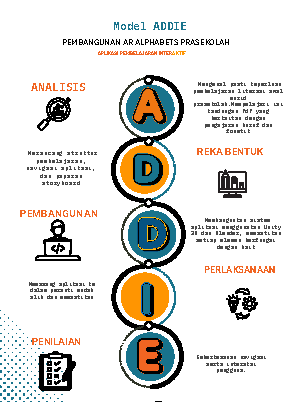
\includegraphics[width=1\linewidth]{MODEL ADDIES.pdf}
    \caption{Model ADDIE}
    \label{fig:enter-addie}
\end{figure}




\section{Unity }
Unity 3D adalah perisian untuk mencipta permainan tiga dimensi yang 
digabungkan untuk menghasilkan animasi tiga dimensi secara masa nyata 
(waktu nyata). Unity dilengkapi dengan Persekitaran Pembangunan Terpadu (IDE) 
dikenali sebagai Mono Develop, yang bertujuan untuk mengintegrasikan semua skrip 
dihasilkan ke dalam Unity, untuk diproses secara langsung. Unity 3D 
dibangunkan oleh Unity Technologies, ditubuhkan pada tahun 2004 oleh David 
Helgason, Nicholas Francis, dan Joachim Ante. Pada tahun 2009, Unity dilancarkan 
secara percuma, dan kini ia telah menarik berjuta-juta pembangun dari seluruh dunia 
untuk mendaftar (Rahmat & Yanti, 2021). Unity menyokong pembangunan aplikasi 
Android. Sebelum aplikasi yang dibina menggunakan Unity untuk Android 
boleh dijalankan, konfigurasi persekitaran pembangunan Android pada peranti adalah  diperlukan. Untuk itu, pembangun perlu memuat turun dan memasang Android SDK.  dan menambah peranti fizikal ke dalam sistem. Unity Android membenarkan memanggil fungsi khas yang ditulis dalam C/C++ secara langsung dan Java secara tidak langsung secara tidak langsung melalui skrip C# (Andriansyah et al., 2019).

\section{Blender}
Software	Description
	Unity 3D adalah perisian untuk mencipta permainan tiga dimensi yang 
digabungkan untuk menghasilkan animasi tiga dimensi secara masa nyata 
(waktu nyata). Unity dilengkapi dengan Persekitaran Pembangunan Terpadu (IDE) 
dikenali sebagai Mono Develop, yang bertujuan untuk mengintegrasikan semua skrip 
dihasilkan ke dalam Unity, untuk diproses secara langsung. Unity 3D 
dibangunkan oleh Unity Technologies, ditubuhkan pada tahun 2004 oleh David 
Helgason, Nicholas Francis, dan Joachim Ante. Pada tahun 2009, Unity dilancarkan 
secara percuma, dan kini ia telah menarik berjuta-juta pembangun dari seluruh dunia 
untuk mendaftar (Rahmat & Yanti, 2021). Unity menyokong pembangunan aplikasi 
Android. Sebelum aplikasi yang dibina menggunakan Unity untuk Android 
boleh dijalankan, konfigurasi persekitaran pembangunan Android pada peranti adalah  diperlukan. Untuk itu, pembangun perlu memuat turun dan memasang Android SDK.  dan menambah peranti fizikal ke dalam sistem. Unity Android membenarkan memanggil fungsi khas yang ditulis dalam C/C++ secara langsung dan Java secara tidak langsung secara tidak langsung melalui skrip C# (Andriansyah et al., 2019).

	\hspace{1cm}Blender merupakan salah satu perisian percuma yang sering dikenali sebagai suite penciptaan 3D sumber terbuka, yang menyokong keseluruhan proses dalam mod tiga dimensi seperti pemodelan, pemasangan rangka, animasi, simulasi, rendering, dan penjejakan gerakan. Malah, perisian ini juga menyokong pembangunan permainan (Valentino, 2017). Pada mulanya, Blender diciptakan sebagai alat pengeluaran dalaman untuk syarikat animasi Belanda yang terkemuka, NeoGeo, yang diasaskan oleh pemaju asal Blender dan masih menjadi pemaju utama hingga ke hari ini, Ton Roosendaal. Menjelang akhir tahun 1990-an, NeoGeo mula menawarkan salinan Blender untuk dimuat turun melalui laman web mereka. Secara perlahan tetapi konsisten, minat terhadap program yang kurang daripada 2 MB ini semakin berkembang. Pada tahun 1998, Ton menubuhkan syarikat baharu, Not a Number (NaN), untuk memasarkan dan menjual Blender sebagai produk perisian. NaN terus menyediakan versi percuma Blender tetapi juga menawarkan versi premium dengan lebih banyak ciri pada harga yang berpatutan. Strategi ini terbukti berkesan, dan pada akhir tahun 2000, pengguna Blender telah mencapai lebih daripada 250,000 di seluruh dunia (Gumster, 2015, hal. 11).
\section{Vuforia}
	Vuforia adalah Kit Pembangunan Perisian (SDK) yang dibangunkan oleh Qualcomm untuk membantu pembangun aplikasi mudah alih dalam mencipta aplikasi Realiti Terimbuh (AR) pada telefon pintar sama ada berasaskan Android atau iOS (Rahmat & Yanti, 2021). SDK Vuforia juga boleh diintegrasikan dengan Unity, dikenali sebagai Vuforia AR Extension for Unity. Vuforia AR Extension membolehkan Unity memaparkan animasi realiti terimbuh yang telah direka sebelumnya (Desierto et al., 2020). Untuk berfungsi dengan optimum, SDK Vuforia memerlukan beberapa komponen penting. Komponen tersebut merangkumi kamera, penukar imej, alat pengesan, rendering latar belakang video, kod aplikasi, trackables, dan marker. Semua komponen ini digunakan dalam pembangunan aplikasi berasaskan AR (Mustaqim, 2017).
\section{Figma}
	Figma merupakan salah satu alat reka bentuk yang sering digunakan untuk mencipta antaramuka aplikasi mudah alih, desktop, laman web, dan banyak lagi. Figma boleh diakses pada sistem operasi Windows, Linux, atau Mac dengan sambungan internet. Keunggulan Figma terletak pada kemampuannya untuk membolehkan lebih dari satu individu berkolaborasi secara serentak, walaupun berada di lokasi yang berbeza. Fenomena ini dapat dianggap sebagai kerja berkumpulan, dan disebabkan oleh keupayaan aplikasi Figma, ia telah menjadi pilihan utama bagi banyak pereka UI/UX untuk menghasilkan prototaip laman web atau aplikasi dengan cara yang cepat dan berkesan (Al-Faruq et al., 2022).
	Adobe Illustrator merupakan aplikasi yang digunakan untuk menyunting reka bentuk grafik dalam penerbitan web dan desktop, serta mampu berintegrasi dengan perisian lain yang relevan (Rian et al., 2021). Adobe Illustrator dapat digunakan untuk menyunting atau mencipta imej dan butang dalam proses pembangunan aplikasi.


\begin{tabular}{>{\raggedright}p{3cm}>{\centering}p{2cm}p{8cm}}
\toprule
\textbf{Aplikasi AR} & \textbf{Logo} & \textbf{Huraian} \\
\midrule
Dinosaur3DAR & 

\includegraphics[width=1.5cm]{dino.pdf}& 
Aplikasi ini dikhuskan kepada penggemar dinosaur.  Aplikasi ini amat sesuai untuk kanak-kanak yang teruja menerokai dunia prasejarah dan mempelajari tentang makhluk purba seperti dinosaur.\\

Earth Zoo AR & 
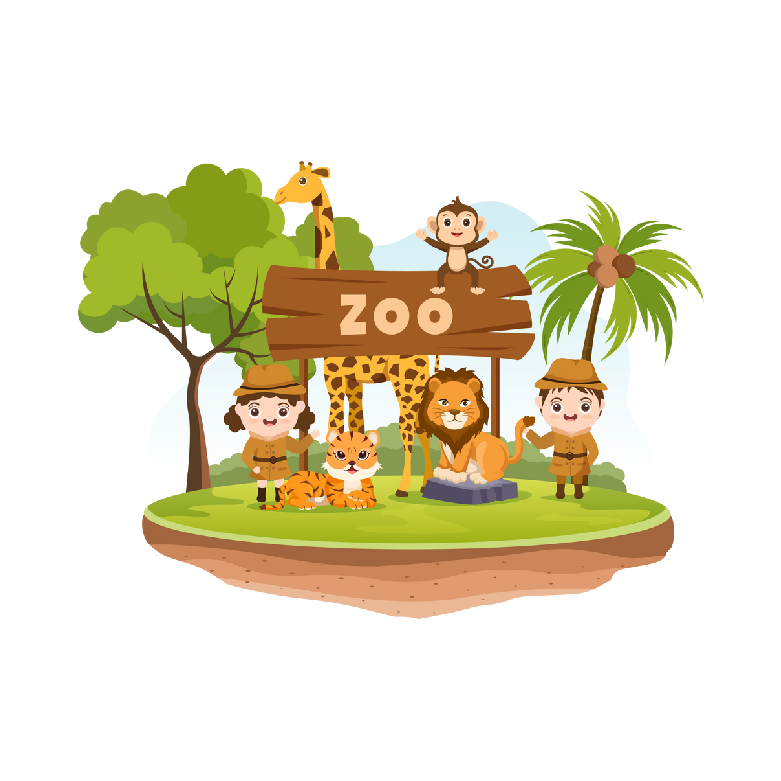
\includegraphics[width=1.5cm]{===200.pdf}& 
 menampilkan objek dalam bentuk 3D. EarthZoo-AR menawarkan pengalaman seolah-olah melawat zoo maya.\\

Kad Flash AR & 
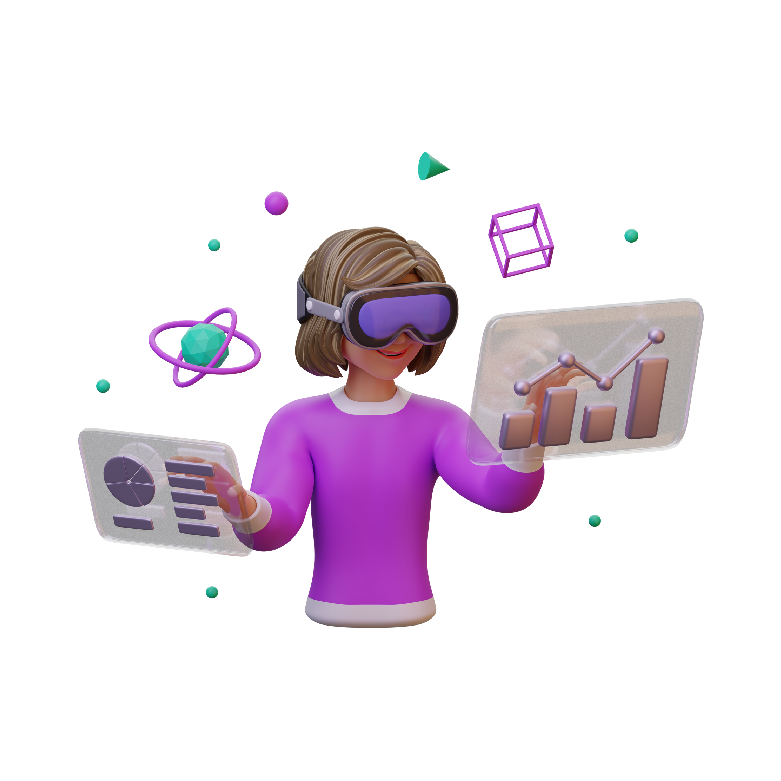
\includegraphics[width=1.5cm]{===300.pdf}& 
Aplikasi ini bertujuan untuk mendidik kanak-kanak melalui kad flash AR. Dengan pemanfaatan teknologi ini, kanak-kanak dapat melihat huruf dan haiwan dalam bentuk 3D sambil mendengar nama serta bunyi haiwan tersebut, m\\

Math ARi & 
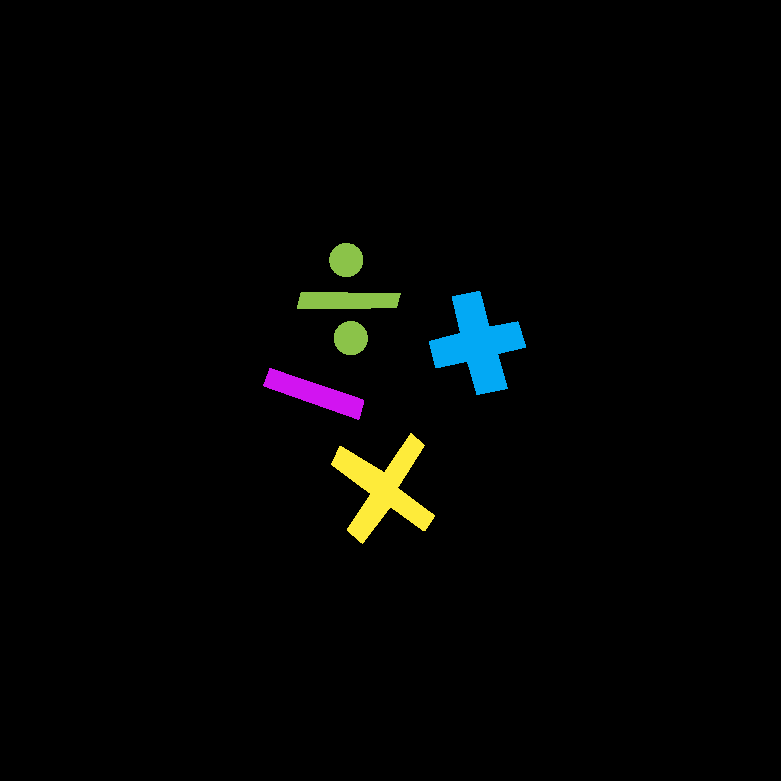
\includegraphics[width=1.5cm]{mate.pdf} & 
Aplikasi ini direka untuk memperkenalkan kanak-kanak kepada asas-asas pembelajaran seperti huruf, nama haiwan, dan kata-kata melalui interaksi AR yang menghiburkan. Ia amat sesuai untuk kanak-kanak kecil kerana pendekatannya yang mudah dan berkesan. \\

AR Paint & 

\includegraphics[width=1.5cm]{zooz1.pdf}& 
Aplikasi kreatif ini membolehkan pengguna menghasilkan hologram 3D, lukisan, dan patung. Ia menawarkan peluang untuk meneroka kreativiti, menyertai komuniti seni maya.\\
\bottomrule
\end{tabular}

\subsection{2.6 Penggunaan UML dalam Pembangunan Aplikasi Pendidikan AR}

Pembangunan aplikasi pendidikan seperti \textit{AR Alphabets} memerlukan perancangan yang sistematik, terutamanya dari aspek kejuruteraan perisian. Salah satu pendekatan yang digunakan ialah penggunaan Unified Modeling Language (UML) bagi memvisualisasikan keperluan sistem dan interaksi antara pengguna dengan sistem. UML membantu dalam dokumentasi proses pembangunan aplikasi, menjadikan reka bentuk lebih jelas dan mudah difahami oleh pembangun.

Dalam konteks aplikasi \textit{AR Alphabets}, beberapa jenis diagram UML telah digunakan:
\begin{itemize}
  \item \textbf{Use Case Diagram} – menunjukkan fungsi sistem dan peranan pengguna.
  \item \textbf{Activity Diagram} – menerangkan urutan aktiviti pengguna semasa menggunakan fungsi tertentu dalam aplikasi.
  \item \textbf{Flowchart} – memvisualisasikan aliran proses untuk setiap modul aplikasi.
\end{itemize}

Rajah-rajah berikut menunjukkan contoh diagram UML yang digunakan dalam aplikasi ini.


\subsection{Teori Tindakan Norman dalam Reka Bentuk Antaramuka Pengguna}

Teori Tindakan oleh Donald Norman (1990) merupakan salah satu teori asas dalam bidang interaksi manusia-komputer (HCI) yang menjelaskan proses mental dan tindakan fizikal yang berlaku apabila pengguna berinteraksi dengan sesuatu sistem atau aplikasi. Teori ini terdiri daripada tujuh peringkat, iaitu: (i) penetapan matlamat (forming the goal), (ii) penetapan niat (forming the intention), (iii) penentuan tindakan (specifying an action), (iv) pelaksanaan tindakan (executing the action), (v) persepsi kesan (perceiving the system state), (vi) pentafsiran kesan (interpreting the system state), dan (vii) penilaian hasil (evaluating the outcome)norman1990}.

Dalam konteks pembangunan aplikasi \textit{AR Alphabets}, teori ini memainkan peranan penting dalam memastikan reka bentuk antaramuka adalah selaras dengan jangkaan dan keperluan pengguna, khususnya murid prasekolah dan guru. Sebagai contoh, apabila murid ingin mengenali huruf, mereka mempunyai matlamat (mengenal huruf), kemudian menetapkan niat (menekan kad AR atau ikon huruf), melaksanakan tindakan tersebut, dan aplikasi akan memberikan maklum balas visual dan audio. Sekiranya aplikasi berjaya membantu murid mencapai matlamat ini dengan mudah, maka jurang tindakan (gulf of execution) dan jurang penilaian (gulf of evaluation) dapat dikurangkan.

\textbf{Jurang Tindakan (Gulf of Execution)} merujuk kepada kesukaran pengguna untuk melaksanakan tindakan yang sesuai dalam sistem. Dalam aplikasi \textit{AR Alphabets}, antaramuka yang intuitif, susunan ikon yang jelas, dan interaksi berasaskan sentuhan membantu murid prasekolah melaksanakan tindakan mereka dengan lebih mudah tanpa kekeliruan.

\textbf{Jurang Penilaian (Gulf of Evaluation)} pula merujuk kepada kesukaran pengguna memahami kesan tindakan mereka. Aplikasi ini meminimumkan jurang tersebut melalui maklum balas segera seperti animasi 3D, bunyi fonetik, dan paparan visual yang menyatakan huruf yang sedang dipelajari. Murid dapat segera menilai bahawa tindakan mereka (menekan butang atau mengimbas kad) telah menghasilkan tindak balas yang tepat.
\subsection{Hubungan Teori Norman dengan Skala SUS dalam Kajian Ini}

Dalam kajian ini, tahap kebolehgunaan aplikasi telah dinilai menggunakan \textit{System Usability Scale (SUS)}, yang mengukur aspek kejelasan, keberkesanan, dan kepuasan pengguna terhadap sistem. Dapatan skor SUS sebanyak 87.5 menunjukkan bahawa aplikasi \textit{AR Alphabets} berada pada tahap kebolehgunaan yang sangat baik.

Teori Norman memperkukuh dapatan ini dengan menjelaskan mengapa aplikasi ini berfungsi dengan baik dari perspektif interaksi pengguna. Reka bentuk antaramuka yang meminimumkan beban kognitif dan membolehkan pengguna mencapai matlamat mereka dengan mudah adalah faktor utama yang menyumbang kepada skor SUS yang tinggi. Dengan kata lain, apabila jurang tindakan dan penilaian dapat diminimumkan melalui reka bentuk sistem yang sesuai, pengguna lebih cenderung untuk berasa puas, memahami fungsi sistem, dan menggunakannya dengan cekap—sejajar dengan elemen-elemen yang diukur dalam SUS.

\begin{figure}[H]
\centering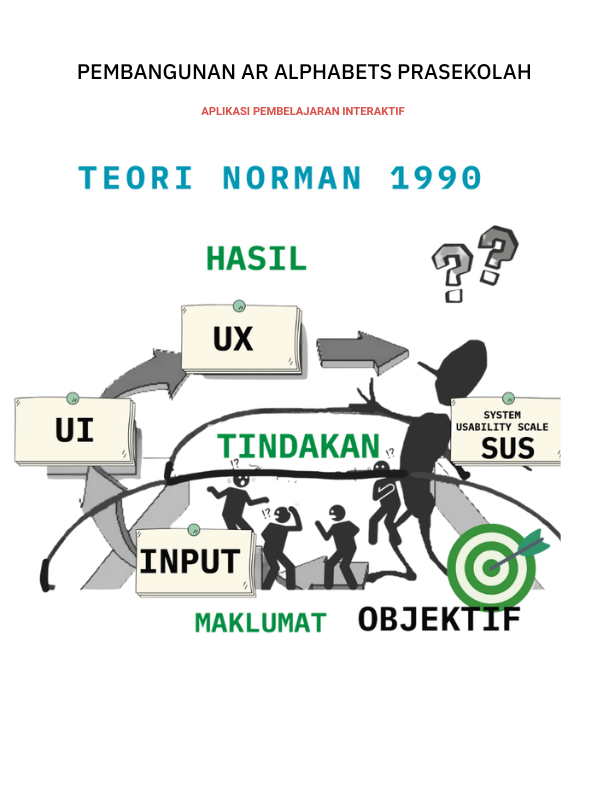
\includegraphics[width=0.8\textwidth]{------norman teori.png}\caption{Model Tindakan Norman dalam Konteks Aplikasi \textit{AR Alphabets} (Disesuaikan daripada Norman, 1990)}\label{rajah:norman}\end{figure}

\subsection{Skala Kebolehgunaan Sistem (System Usability Scale, SUS)}

Dalam usaha menilai sejauh mana kejayaan sesuatu sistem atau aplikasi, satu bentuk pengukuran yang kerap digunakan ialah Skala Kebolehgunaan Sistem atau \textit{System Usability Scale} (SUS). SUS merupakan satu instrumen soal selidik yang dibangunkan oleh John Brooke pada tahun 1986 bagi menilai aspek kebolehgunaan pelbagai jenis produk dan sistem termasuk aplikasi mudah alih, laman sesawang, dan perisian interaktif (brooke, 1986).

Terdapat beberapa ciri unik SUS yang menjadikannya salah satu alat penilaian yang paling popular dan praktikal dalam kajian pengalaman pengguna. Pertama, SUS hanya terdiri daripada sepuluh item soalan, menjadikannya mudah dan cepat untuk dijawab oleh responden {Kedua, SUS bersifat agnostik teknologi, membolehkannya digunakan untuk menilai hampir semua jenis antara muka seperti laman sesawang, aplikasi telefon pintar, sistem maklum balas suara (IVR), sistem berasaskan sentuhan, dan lain-lain . Ketiga, hasil soal selidik ini dikira menjadi satu skor tunggal antara 0 hingga 100, yang mudah difahami oleh pengguna dari pelbagai latar belakang teknikal mahupun bukan teknikal (brooke, 1986).

\begin{figure}[H]   
\centering    \includegraphics[width=0.8\textwidth]{Screenshot 2025-07-05 at 1.16.03 AM.png}    \caption{Skor SUS Berdasarkan Kategori Penilaian \cite{bangor2009determining}}    \label{fig:sus-score}\end{figure}

Skor SUS yang diperoleh biasanya ditafsir mengikut julat berikut:

\begin{itemize}    \item \textbf{Grade A (Sangat Baik)}: Skor $\geq$ 84    \item \textbf{Grade B (Baik)}: Skor antara 72 hingga kurang daripada 84    \item \textbf{Grade C (Memuaskan)}: Skor antara 53 hingga kurang daripada 72    \item \textbf{Grade D (Kurang Memuaskan)}: Skor antara 39 hingga kurang daripada 53    \item \textbf{Grade F (Tidak Memuaskan)}: Skor $<$ 39\end{itemize}

Melalui analisis SUS, penyelidik dapat menilai secara kuantitatif tahap kebolehgunaan sistem serta mengenal pasti keperluan penambahbaikan dalam reka bentuk antara muka pengguna.

Kesimpulannya, integrasi Teori Tindakan Norman dalam reka bentuk \textit{AR Alphabets} bukan sahaja memperkukuh aspek reka bentuk antaramuka, malah menyokong justifikasi keberkesanan aplikasi berdasarkan dapatan ujian SUS. Ia menjadikan pengalaman pengguna lebih intuitif dan bermakna, terutama bagi murid prasekolah yang memerlukan pembelajaran yang menyeronokkan serta mudah difahami.